\documentclass{article}
\usepackage{graphicx}
\graphicspath{{images/}}

\title{The answer is 42}
\author{Nasser Alshammari}
\date{Feb 2016}

\begin{document}

\maketitle

\section{Introduction}
Aliquam erat volutpat.  Nunc eleifend leo vitae magna.  In id erat non orci commodo lobortis.  Proin neque massa, cursus ut, gravida ut, lobortis eget, lacus.  Sed diam.  Praesent fermentum tempor tellus.  Nullam tempus.  Mauris ac felis vel velit tristique imperdiet.  Donec at pede.  Etiam vel neque nec dui dignissim bibendum.  Vivamus id enim.  Phasellus neque orci, porta a, aliquet quis, semper a, massa.  Phasellus purus.  Pellentesque tristique imperdiet tortor.  Nam euismod tellus id erat.


\section{Background}
Lorem ipsum dolor sit amet, consectetuer adipiscing elit.  Donec hendrerit tempor tellus.  Donec pretium posuere tellus.  Proin quam nisl, tincidunt et, mattis eget, convallis nec, purus.  Cum sociis natoque penatibus et magnis dis parturient montes, nascetur ridiculus mus.  Nulla posuere.  Donec vitae dolor.  Nullam tristique diam non turpis.  Cras placerat accumsan nulla.  Nullam rutrum.  Nam vestibulum accumsan nisl.

\subsection{Hitchhiking in the galaxy}
Nullam tristique diam non turpis. Vestibulum convallis, lorem a tempus semper, dui dui euismod elit, vitae placerat urna tortor vitae lacus.  Etiam vel neque nec dui dignissim bibendum. 

\subsubsection{Do not panic}
Fusce sagittis, libero non molestie mollis, magna orci ultrices dolor, at vulputate neque nulla lacinia eros. Nam a sapien.  Vestibulum convallis, lorem a tempus semper, dui dui euismod elit, vitae placerat urna tortor vitae lacus.   

\subsection{The guide to Hitchhiking}
Phasellus at dui in ligula mollis ultricies. Nullam tristique diam non turpis.  Nam vestibulum accumsan nisl.  Fusce commodo.  Etiam vel tortor sodales tellus ultricies commodo.   

\section{Methodology}
Lorem ipsum dolor sit amet, consectetuer adipiscing elit.  Donec hendrerit tempor tellus.  Donec pretium posuere tellus.  Proin quam nisl, tincidunt et, mattis eget, convallis nec, purus.  Cum sociis natoque penatibus et magnis dis parturient montes, nascetur ridiculus mus.  Nulla posuere.  Donec vitae dolor.  Nullam tristique diam non turpis.  Cras placerat accumsan nulla.  Nullam rutrum.  Nam vestibulum accumsan nisl.

To write simple math: $1 + 2 = 4$ or something like this $\alpha + \beta = \epsilon$

\begin{equation}
\sin(x) = 0.45 
\end{equation}

Lorem ipsum dolor sit amet, consectetuer adipiscing elit.  Donec hendrerit
tempor tellus.  Donec pretium posuere tellus.  Proin quam nisl, tincidunt et,
mattis eget, convallis nec, purus.  

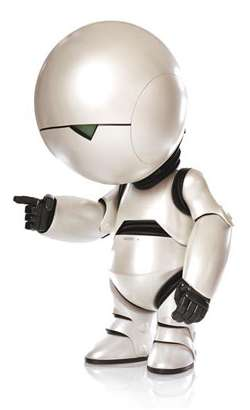
\includegraphics[height=3cm]{marvin}

Cum sociis natoque penatibus et magnis dis parturient montes, nascetur ridiculus mus.  Nulla posuere.  Donec vitae dolor.  Nullam tristique diam non turpis.  Cras placerat accumsan nulla.  Nullam rutrum.  Nam vestibulum accumsan nisl.


\end{document}